\documentclass{article}
\usepackage{nips10submit_e,times}
%\documentstyle[nips07submit_09,times]{article}
\usepackage[square,numbers]{natbib}
\usepackage{amsmath, epsfig}
\usepackage{amsfonts}
\usepackage{subfigure}
\usepackage{graphicx}
\usepackage{amsfonts}
\usepackage{algorithm}
\usepackage{algorithmic}
\usepackage{easybmat}
\usepackage{footmisc}
\renewcommand\algorithmiccomment[1]{// \textit{#1}}
%
\newcommand{\ignore}[1]{}
\newcommand{\comment}[1]{}
\DeclareMathOperator*{\argmax}{arg\,max}

\title{Awesome Project Using Machine Learning}


\author{
Student One \hspace{1cm} Student Two \hspace{1cm} Student Three \hspace{1cm} Frank Wood\\
Columbia University, New York, NY 10027, USA \\
\texttt{\{stud1@otherdepth.,\{stud3,fwood\}@stat.,\{stud2\}@columbia.edu}
%\texttt{pfau@neurotheory.columbia.edu} 
%\texttt{\{bartlett,fwood\}@stat.columbia.edu} 
}

% The \author macro works with any number of authors. There are two commands
% used to separate the names and addresses of multiple authors: \And and \AND.
%
% Using \And between authors leaves it to \LaTeX{} to determine where to break
% the lines. Using \AND forces a linebreak at that point. So, if \LaTeX{}
% puts 3 of 4 authors names on the first line, and the last on the second
% line, try using \AND instead of \And before the third author name.

\newcommand{\fix}{\marginpar{FIX}}
\newcommand{\new}{\marginpar{NEW}}
\newcommand{\X}{\mathcal{X}}


\nipsfinalcopy

\begin{document}

\maketitle

\begin{abstract}
This paper presents an awesome idea in my field for which the answer was unknown but now I know how to solve it using tools from statistical machine learning.  
\end{abstract}

\section{Introduction}
\label{sec:introduction}
This is your introduction.  You might say something about Fig.~\ref{fig:example} which has something to do with the work of \citep{Wood2009}
\section{Methods}
These are the methods you use.  You'll probably have some horrible equations in this section like

\begin{equation}
P(\Theta|\X) \propto P(\X|\Theta) P(\Theta) % note that \X is defined above
\label{eqn:bayes_rule}
\end{equation}

And you might want to include a figure.  Note that this figure floats around on its own.  Don't worry about layout.  Notice that the figure doesn't appear where you put it.  That's OK.  Things will look OK when there is enough material in the paper.

\begin{figure}[htbp] %  figure placement: here, top, bottom, or page
   \centering
   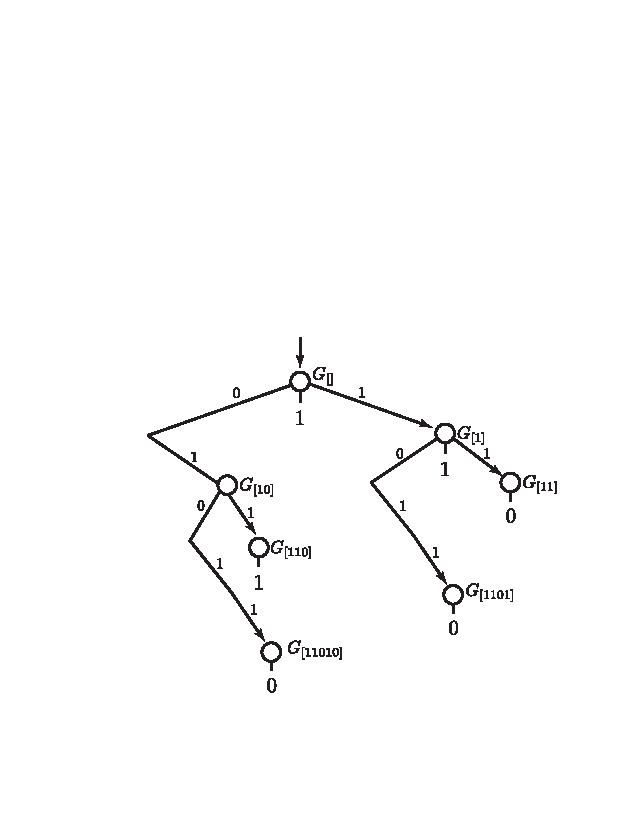
\includegraphics[width=4in]{fig1} 
   \caption{example caption}
   \label{fig:example}
\end{figure}

You might want to refer to Bayes Rule (Eqn.~\ref{eqn:bayes_rule}) in the text.

\section{Experiments}

Here is where your awesome experiments go.

\section{Conclusion}

Presumably you'll have something smart to say here.

\begin{small}
\bibliographystyle{plainnat}
\bibliography{refs} 
\end{small}
\end{document}
